\documentclass{article}
\usepackage[utf8]{inputenc}
\usepackage{amsfonts}
\usepackage{graphicx}
\usepackage{caption}
\usepackage{geometry}
\usepackage{subcaption}
\usepackage{booktabs,siunitx,array,threeparttable}
\usepackage{listings}
\usepackage{xcolor}
\usepackage{pdfpages}
\usepackage{cite}

\geometry{
 a4paper,
 total={170mm,257mm},
 left=20mm,
 top=20mm,
 }

\title{Report for Assignment 3}
\author{2053814 }
\date{November 2022}

\setlength\parindent{0pt}

\begin{document}

\maketitle

\definecolor{codegreen}{rgb}{0,0.6,0}
\definecolor{codegray}{rgb}{0.5,0.5,0.5}
\definecolor{codepurple}{rgb}{0.58,0,0.82}
\definecolor{backcolour}{rgb}{0.95,0.95,0.92}

\lstdefinestyle{mystyle}{
    backgroundcolor=\color{backcolour},   
    commentstyle=\color{codegreen},
    keywordstyle=\color{magenta},
    numberstyle=\tiny\color{codegray},
    stringstyle=\color{codepurple},
    basicstyle=\ttfamily\footnotesize,
    breakatwhitespace=false,         
    breaklines=true,                 
    captionpos=b,                    
    keepspaces=true,                 
    numbers=left,                    
    numbersep=5pt,                  
    showspaces=false,                
    showstringspaces=false,
    showtabs=false,                  
    tabsize=2
}
\lstset{style=mystyle}

\newcommand*\sepline{%
  \begin{center}
    \rule[1ex]{\textwidth}{.5pt}
  \end{center}}

\section{Introduction}

The report are divided into two parts:

\begin{enumerate}
    \item Investigated Taylor's Series, including the proof, general application, accuracy, especially about simplify functions and calculate numeric integral,
    \item Investigated method of finding zero points of a function. Including bisection, fixed-point and Newton's method. Also concerning their convergence rate and (dis-)advantages.
\end{enumerate}

These numeric method has different behavior in different situation, and in computer science, analytical solutions usually hard to compute and even don't exist, hence develop numeric method and apply them at proper time is important.

Besides, as a student, doing some exampling and experiments is helpful to get a comprehensive understanding of a problem. 


\section{Polynomial Approximations}

\subsection{Overview}

For a function $f\in C^n[a,b]$, it may be expanded to 

$$f(x) = \sum_{k=0}^{n-1}\frac{f^{(k)}(x_0)}{k!}(x-x_0)^k + \frac{f^{(n}(\zeta)}{n!}(x-x_0)^n,\quad \zeta\in[\min(x,x_0),\max(x,x_0)]$$

at $x=x_0$. This is called Taylor's Series. It approximates a continuous enough function, no matter it has an analytical expression or not, or how complicated it is, by a series of polynomials, which is easy to handle. And besides, it's rounding error is easy to calculate and manipulate: 
$$E(f)=\frac{f^{(n)}(\zeta)}{n!}(x-x_0)^n,\quad \zeta\in[\min(x,x_0),\max(x,x_0)]$$
if we expand it to the $n$-th item.
$$\hat{f}_n(x)=\sum_{k=0}^{n-1}\frac{f^{(k)}(x_0)}{k!}(x-x_0)^k$$
For example, we can use the first several items of $\sin x$'s Taylor Series at $x=x_0=0$, i.e.\cite{sintaylor}
$$\sin(x)=x-\frac{1}{3!}x^3+\frac{1}{5!}x^5+\cdot+(-1)^{n}\frac{1}{(2n+1)!}x^{2n+1}+\cdots$$
to compute $\sin x$ approximately, and the smaller $|x-x_0|$ is, the more accurate results we could get.
Take $x=0.01$, pick the first 4 items, we can get
$$\sin 0.01\approx 0.01-\frac{1}{3!}0.01^3+\frac{1}{5!}0.01^5-\frac{1}{7!}0.01^7\approx 9.99983\time10^{-3}$$
and we can verify that the relative error is $2.76\times 10^{-22}$, it's pretty good.
Approximation is important especially when we need to simplify complex problems and expressions, and high-order details can be neglected.

\subsection{Proof}

Here we shall give a brief prove for it.

Consider the following expansion of $f(x)\in C^{(n+1)}(\mathbb{R})$, we have

$$\begin{array}{rl}
f(x)&=\displaystyle f(0)+\int_0^x f'(t)dt\\
&\displaystyle=f(0)+f'(0)x+\int_0^x tf''(x-t)dx\\
&\displaystyle=f(0)+f'(0)x+\frac{1}{2}f''(0)x^2+\frac{1}{2}\int_0^x t^2f'''(x-t)dt\\
&\displaystyle=\sum_{k=0}^n \frac{f^{(n)}(0)}{n!}x^n+\frac{1}{n!}\int_{0}^x t^nf^{(n+1)}(x-t)dt\\
&\displaystyle=\sum_{k=0}^n \frac{f^{(n)}(0)}{n!}x^n+\frac{f^{(n+1)}(\zeta)}{(n+1)!}x^{n+1}
\end{array}$$

translate $f(x)$ by a, i.e. let $t-a=x$, then 

$$f(t)=\sum_{k=0}^n \frac{f^{(n)}(a)}{n!}(t-a)^n+\frac{f^{(n+1)}(\zeta)}{(n+1)!}(t-a)^{n+1}$$

\subsection{Example}

Let $\displaystyle f(x)=\ln\left|\sin\left(x+\frac{\pi}{2}\right)\right|$, then near $x=0$, we have

$$f'(x)=-\tan x,\quad f''(x)=-(\sec x)^2,\quad f'''(x)=-2(\sec x)^2\tan x\\
f^{(4)}(x)=2(\sec x)^4(\cos 2x-2),\quad f^{(5)}(x)=2(\sec x)^5(\sin 3x - 11\sin x)\\
f^{(6)}(x)=-2(33-26\cos 2x+\cos 4x)(\sec x)^6
$$

Hence, $f(0)=0, f'(0)=0, f''(0)=-1, f'''(0)=0, f^{(4)}(0)=-2, f^{(5)}(0)=0, f^{(6)}(0)=-16$, therefore

$$f(x)\approx \hat{f}(x)=\sum_{k=0}^6\frac{f^{(k)}(x)}{k!}(x-0)^k=-\frac{1}{2}x^2-\frac{1}{12}x^4+-\frac{1}{45}x^6$$

residual $o(x^6)$.

\subsection{Plot}

We plotted Taylor series up to degree 14, and the graphs are like this:

\begin{figure}
    \begin{minipage}{.5\textwidth}
        \centering
        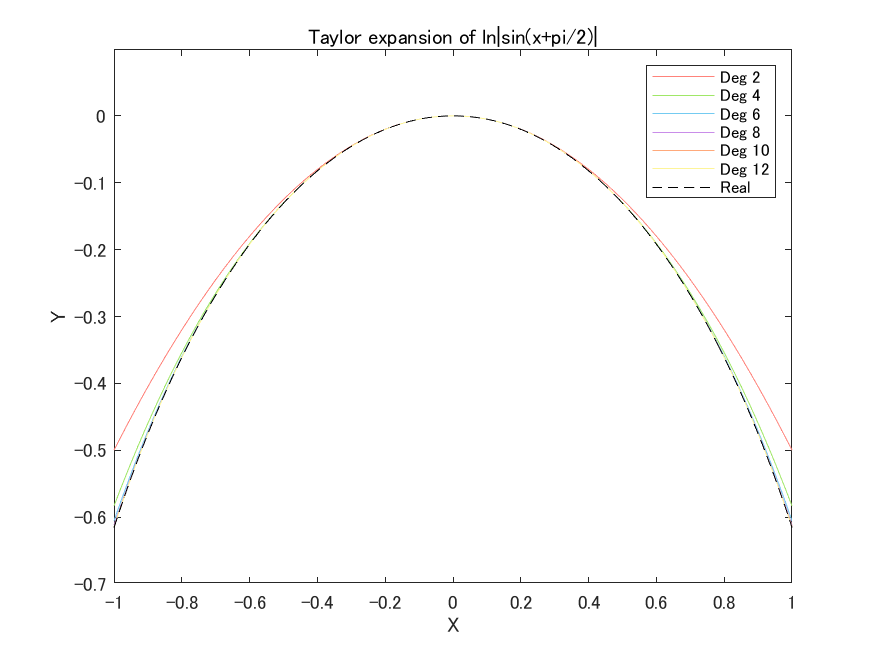
\includegraphics[keepaspectratio,width=.98\linewidth]{taylor-graph.png}
        \caption{Graph of Taylor expansions}
    \end{minipage}
    \begin{minipage}{0.5\textwidth}
        \centering
        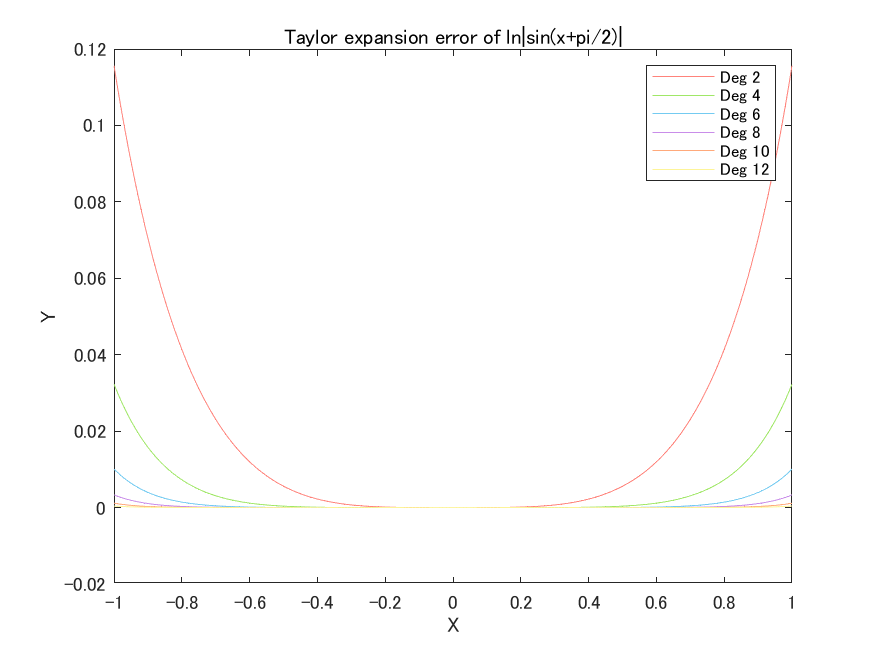
\includegraphics[keepaspectratio,width=.98\linewidth]{taylor-error.png}
        \caption{Error of the approximation}
    \end{minipage}
\end{figure}

So we can see that,

\begin{enumerate} 
    \item the higher the degree is,
    \item the closer $x$ is to $x_0$,
\end{enumerate}

the more accurate our approximation is.

\subsection{Integral}

To calculate 
$$I(f)=\int_{-c}^c -\ln|\sin(x+\pi/2)|dx,\quad c=\frac{(20+a+b)\pi}{90}, a=4,b=1$$

as $\displaystyle c=\frac{5\pi}{18}\pi\approx0.8727$, according to the error graph, the error is monotonously decreasing under $x=0$ and increasing above $x=0$. Since at $x=0.89$, the error is $2.18\times 10^{-4}$, hence our integral will have error less than $3.36\times 10^{-4}$. Anyway, we'll test the actual error of the integral.

\begin{figure}
    \begin{minipage}{.5\textwidth}
        \centering
        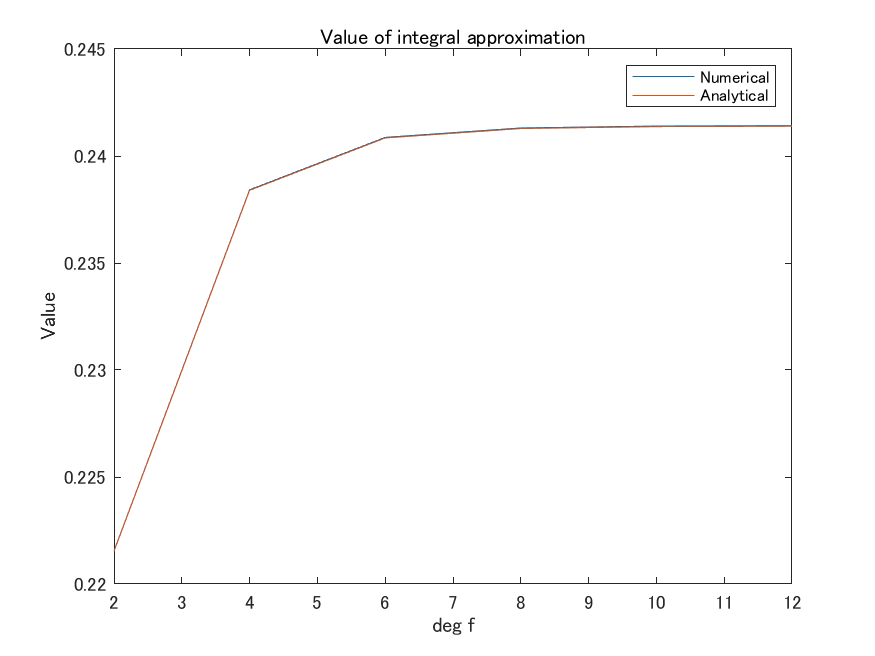
\includegraphics[keepaspectratio,width=.98\linewidth]{taylor-integral-value.png}
        \caption{Graph of value of the integral}
    \end{minipage}
    \begin{minipage}{0.5\textwidth}
        \centering
        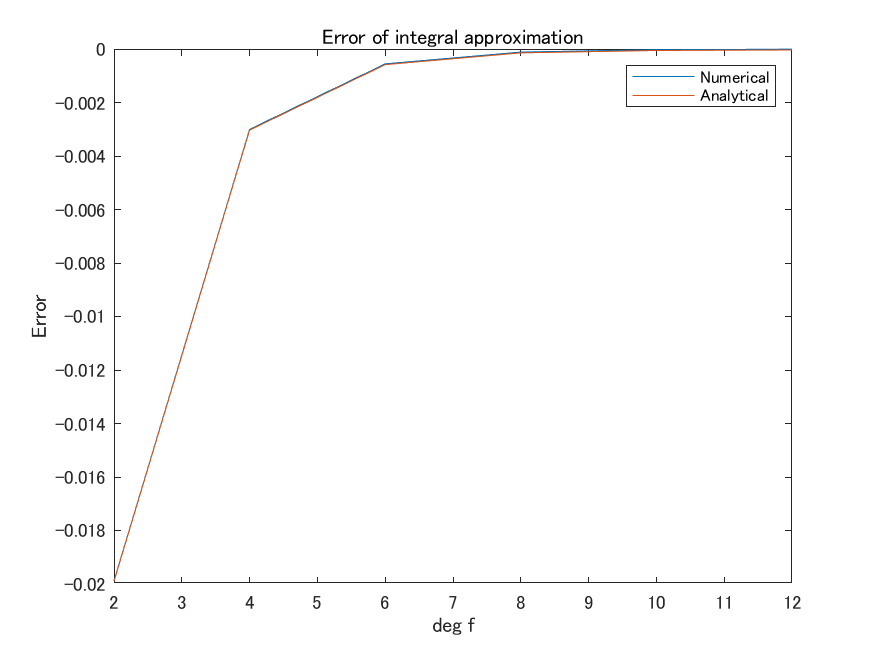
\includegraphics[keepaspectratio,width=.98\linewidth]{taylor-integral-error.png}
        \caption{Error of the approximation of the integral}
    \end{minipage}
\end{figure}

\begin{table}[htbp]
\centering
\begin{threeparttable}
\begin{tabular}{lcccc}
    \toprule
    Degree & Value (Numeric) & Error (Numeric) & value (Analytical) & Error (Analytical) \\
    \midrule
    Degree 2  &   0.221550978320438  &    -0.0198755138374717    &0.221524038925324    &   -0.0199024532325848 \\
    Degree 4  &   0.238424417933728   &  -0.00300207422418164    &0.238394059214865   &   -0.00303243294304412 \\
    Degree 6  &   0.240872208553729  &  -0.000554283604180028   &  0.24084115543027   &   -0.00058533672763969 \\
    Degree 8  &   0.241312378754541  &  -0.000114113403367894    &0.241281165093353   &  -0.000145327064556111 \\
    Degree 10  &  0.241401296952582   & -2.51952053271776e-05 &   0.241370043657112   &  -5.64485007969184e-05 \\
    Degree 12  &  0.241420649687486  &  -5.84247042290098e-06   &  0.24138938619796   &  -3.71059599493517e-05 \\
    \bottomrule
\end{tabular}
\caption{Value and errors of integral using Taylor Series of different order}
\end{threeparttable}
\end{table}

In this table, we used two method to calculate the approximate integral:

$$I(f)=-\int_{-c}^{c}\sum_{k=0}^{n} c_k x^k=\sum_{k=0}^n \frac{c_k}{k+1}(c^{k+1}-(-c)^{k+1})\quad \text{(Analytical)}$$

and

$$I(f)=-\int_{-c}^{c}\sum_{k=0}^{n} c_k x^k=\sum_{k=0}^n \sum_{i=0}^m c_kx_i^k\quad \text{(Numerical)}$$

where $-c\leq x_0<x_1<\cdots<x_n\leq c$ are integral knots. 

As we can see, as the degree of polynomial increases, the error is dropping. And the final result is about $0.24142$, error $3.72\times 10^{-5}$, which is obtained by 12-order Taylor Series expansion.

\section{Finding roots}

Student number 2053814, hence $a=1,b=4$. 
$$x^3+x^2-x+4=0\qquad (1)$$

Let $f(x)=x^3+x^2-x+4$, then $f'(x)=3x^2+2x-1$, $\displaystyle f'(x)=0\to x=-1,\frac{1}{3}$, since $\displaystyle f(\frac{1}{3})=\frac{103}{27}>0$, $f(-1)=5>0$, hence $f(x)$ has only one zero point (*).

\subsection{Bisection method}

\emph{Advantage}: Quick convergence, easy to implement, function no need to be differentiable, stable stepping (interval halved every turn).

\emph{Disadvantage}: Have to determine the approximate interval that a zero point lies in; request the function to be continuous at least, rely on initial values and can only find 1 zero point every time. 

\sepline

This method requires us to find a positive and negative initial value first. Obviously, by (*), we can take a large interval. Then do the following procedure\cite{bisection}:

\begin{lstlisting}[language=R, caption=Bisection Algorithm]
# INPUT: Function f, 
#        endpoint values a, b, 
#        tolerance TOL, 
#        maximum iterations NMAX
# CONDITIONS: a < b, 
#             either f(a) < 0 and f(b) > 0 or f(a) > 0 and f(b) < 0
# OUTPUT: value which differs from a root of f(x) = 0 by less than TOL
 
N <- 1
while N <= NMAX do # limit iterations to prevent infinite loop
    c <- (a + b)/2 # new midpoint
    if f(c) = 0 or (b - a) / 2 < TOL then # solution found
        return (c)
        Stop
    end if
    N <- N + 1 # increment step counter
    if sign(f(c)) = sign(f(a)) then a <- c else b <- c # new interval
end while
\end{lstlisting}

Since the length of the active interval is halved every turn, the time complexity is $O(-\log e)$, $e$ is the given error.\par


\subsection{Fixed point iteration}

\emph{Advantage}: Quick convergence (exponential), easy to implement, stable stepping (interval factored by a variable that has upper bound less than 1 every turn).

\emph{Disadvantage}: Really hard to construct a convergent $\varphi$ function, have to analysis convergence for a selected $\varphi$ and initial value.

\sepline

Fixed-point iteration is a method of computing fixed points of a function.\cite{fixedpoint}

More specifically, given a function ${\displaystyle f}$ defined on the real numbers with real values and given a point ${\displaystyle x_{0}}$ in the domain of $\displaystyle f$, the fixed-point iteration is

$$\displaystyle x_{n+1}=f(x_{n}),\,n=0,1,2,\dots $$

which gives rise to the sequence $\displaystyle x_{0},x_{1},x_{2},\dots $ of iterated function applications $\displaystyle x_{0},f(x_{0}),f(f(x_{0})),\dots $ which is hoped to converge to a point $\displaystyle x_{\rm {fix}}$. If $\displaystyle f$ is continuous, then one can prove that the obtained $\displaystyle x_{\rm {fix}}$ is a fixed point of $\displaystyle f$, i.e.

$$\displaystyle f(x_{\rm {fix}})=x_{\rm {fix}}.$$

By the fixed-point theorem, the algorithm converges to $x'$ for a proper initial value iff. $\exists |C|<1, |x_{n+1}-x_0|<C|x_n-x_0|$.

Detailed procedure

\begin{lstlisting}[language=R, caption=Fixed point Algorithm]
# INPUT: Function phi, 
#        initial value x0
#        tolerance TOL, 
# CONDITIONS: |phi'(fixed_point)| < C < 1
# OUTPUT: fixed point of phi

x0 <- max_float
while abs(x0 - x1) > TOL do # constant C guaranteed convergence
    x0 <- x1
    x1 <- phi(x1)
end while
\end{lstlisting}

For this specific problem, we can take 

$$\varphi(x)=\frac{x-4}{x^2}-1$$

then at the zero point $x_0\in[-2.4,-2.2]$, we have $|\varphi(x_0)|<0.96<1$, so the algorithm will converge, since

$$x_{n+1}=\varphi(x_n)=\varphi(x_0)+\varphi'(x_0)(x_n-x_0)+o(|x_n-x_0|)$$
$$\Rightarrow |x_{n+1}-x_0|<|\varphi'(x_0)||x_n-x_0|<0.99|x_n-x_0|$$

\subsection{Newton's Method}

\emph{Advantage}: Quick convergence (exponential), easy to implement, stable stepping (As a special Fixed point iteration), sometimes the initial values can be taken casually for some good function.

\emph{Disadvantage}: Require the function to be differentiable, not easy to handle function vibrating at high frequency (large tangent), sometimes cannot converge and jump between points.

\sepline

Newton's method is a root-finding algorithm which produces successively better approximations to the roots (or zeroes) of a real-valued function. \cite{newton}

Geometrically, $(x_{n+1}, 0)$ is the intersection of the x-axis and the tangent of the graph of f at $(x_0, f(x_0))$, The process is repeated as

$$\displaystyle x_{n+1}=x_{n}-{\frac {f(x_{n})}{f'(x_{n})}}$$

until a sufficiently precise value is reached. As we can see, let $\displaystyle \varphi(x)=x-\frac{f(x)}{f'(x)}$, then the iteration formula is $x_{n+1}=\varphi{x_n}$, indicating that newton's method is a special case of fixed-point method, therefore the procedure is the same as that method.

For this specific problem, since $f'(x)=3x^2+2x-1$, the iteration formula will be:

$$x_{n+1}=x_n-\frac{x_n^3+x_n^2-x_n+4}{3x_n^2+2x_n-1}$$

\subsection{Result}

Plot for the function and 3 method:

\begin{figure}
    \begin{minipage}{.5\textwidth}
        \centering
        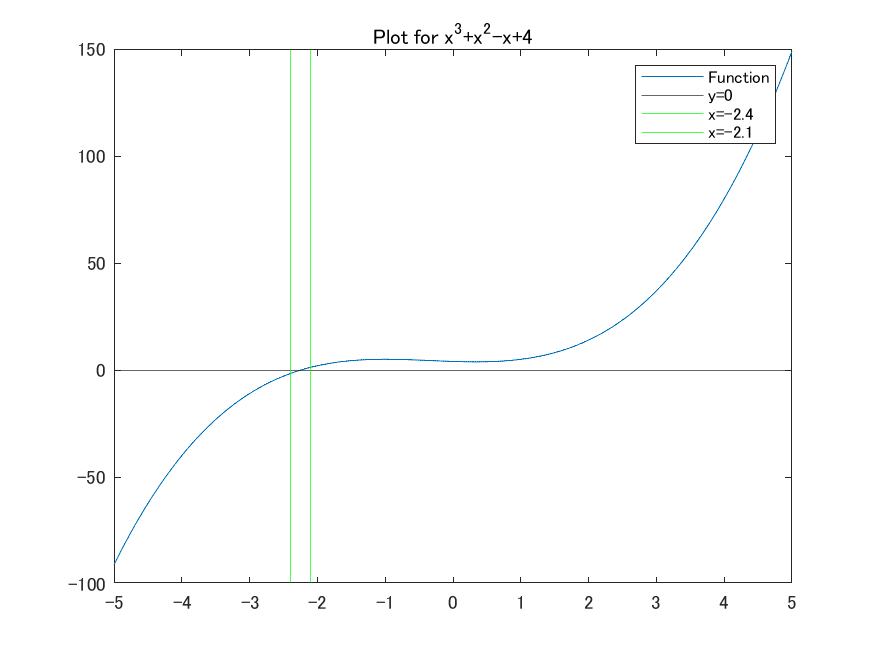
\includegraphics[keepaspectratio,width=.98\linewidth]{function.png}
        \caption{Graph of the function}
        \label{figfunc}
    \end{minipage}
    \begin{minipage}{0.5\textwidth}
        \centering
        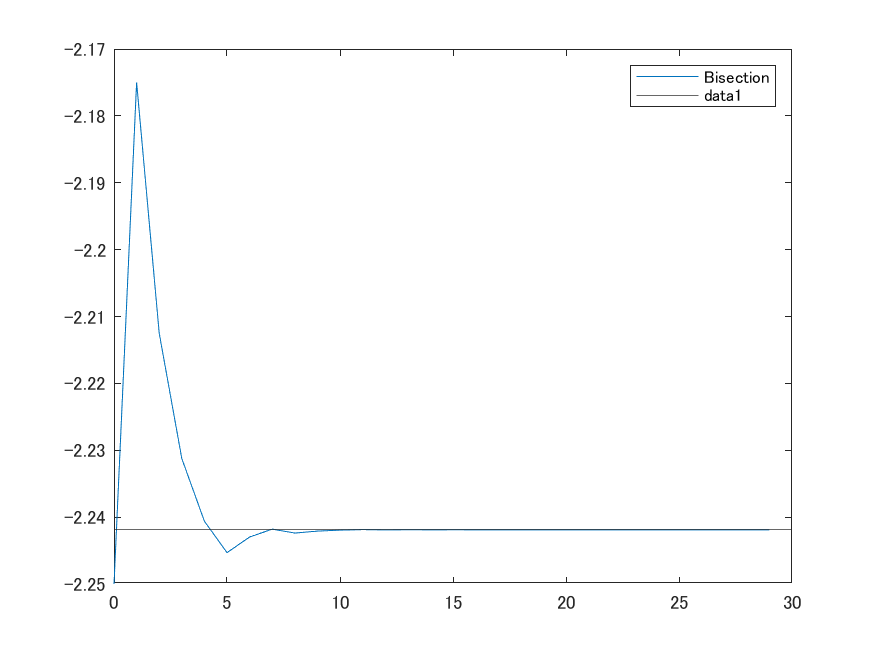
\includegraphics[keepaspectratio,width=.98\linewidth]{Bisection.png}
        \caption{Value of bisection method iteration points}
    \end{minipage}
        \begin{minipage}{0.5\textwidth}
        \centering
        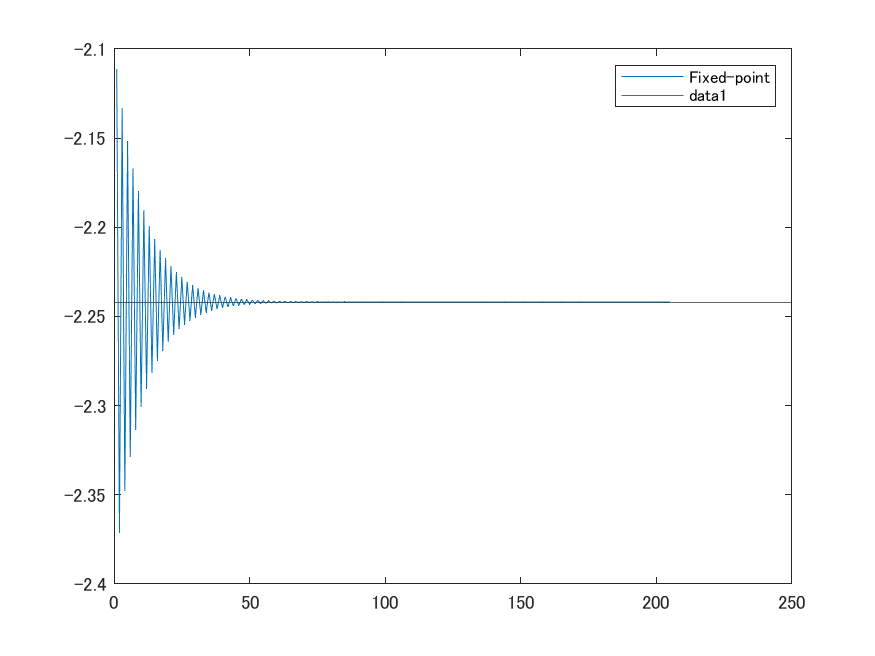
\includegraphics[keepaspectratio,width=.98\linewidth]{Fixed-point.png}
        \caption{Value of fixed point method iteration points}
    \end{minipage}
        \begin{minipage}{0.5\textwidth}
        \centering
        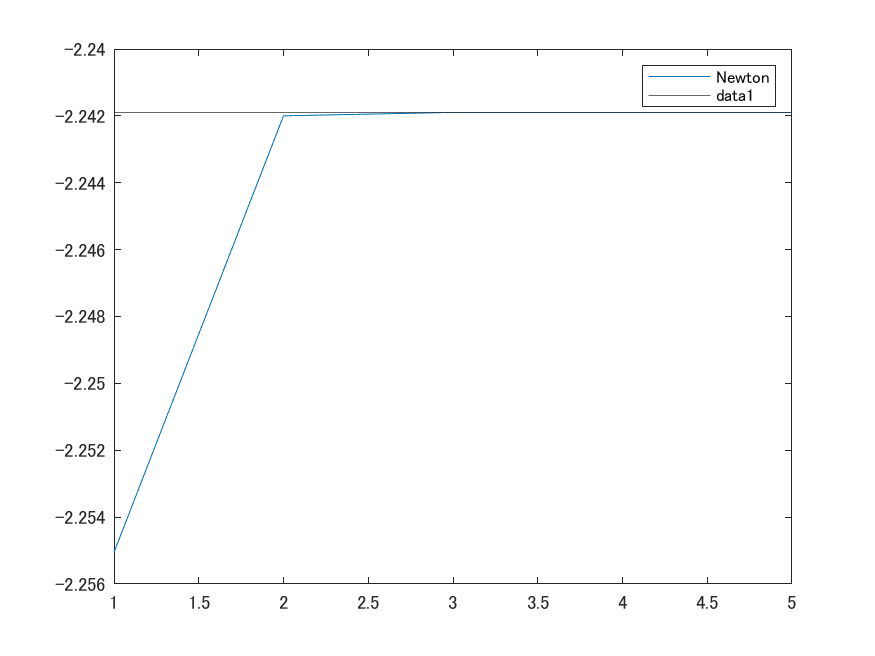
\includegraphics[keepaspectratio,width=.98\linewidth]{Newton.png}
        \caption{Value of Newton's method iteration points}
    \end{minipage}
\end{figure}

From Figure \ref{figfunc}, we can see that $f(x)$ has only one zero point, lying between $-2.4$ to $-2.1$. Hence we can take

\begin{enumerate}
    \item $[-2.4,-2.1]$ as the initial interval for bisection method;
    \item $-2.4$ as the initial value for fixed-point and Newton's Method.
\end{enumerate}

\begin{table}[htbp]
\centering
\begin{threeparttable}
\begin{tabular}{ccc}
    \toprule
    Solution & Function Value & Iterations \\
    \midrule
    -2.24189656303448 &   -1.77635683940025e-15   &     5     \\
    \bottomrule
\end{tabular}
\caption{Result of Newton's Method}
\end{threeparttable}
\end{table}

\begin{table}[htbp]
\centering
\begin{threeparttable}
\begin{tabular}{ccc}
    \toprule
    Solution & Function Value & Iterations \\
    \midrule
    -2.24189656256146 &   4.53838211456059e-09     &  205   \\ 
    \bottomrule
\end{tabular}
\caption{Result of Fixed-point Method}
\end{threeparttable}
\end{table}

\begin{table}[htbp]
\centering
\begin{threeparttable}
\begin{tabular}{ccc}
    \toprule
    Solution & Function Value & Iterations \\
    \midrule
    -2.24189656303448 &   -1.77635683940025e-15   &     29    \\
    \bottomrule
\end{tabular}
\caption{Result of Bisection Method}
\end{threeparttable}
\end{table}

From these tables (table 4 on next page), we can conclude that

\begin{enumerate}
    \item The unique zero point of $f(x)$ is $-2.241896563$, absolute error $10^{-8}$.
    \item Convergence rate: Newton's $>$ Bisection $>$ Fixed point (Note the conclusion not necessarily hold for other situations. )
\end{enumerate}





\newpage

%\begin{thebibliography}{99}  
%
%\bibitem{bisection} Bisection method, Wikipedia, https://en.wikipedia.org/wiki/Bisection
%\bibitem{fixedpoint} Fixed-point iteration, Wikipedia, https://en.wikipedia.org/wiki/Bisection
%\bibitem{newton} Newton's method, Wikipedia, https://en.wikipedia.org/wiki/Newton%27s_method
%
%\end{thebibliography}
\bibliography{ref}{}
\bibliographystyle{plain}

\section{Appendix}

Codes:

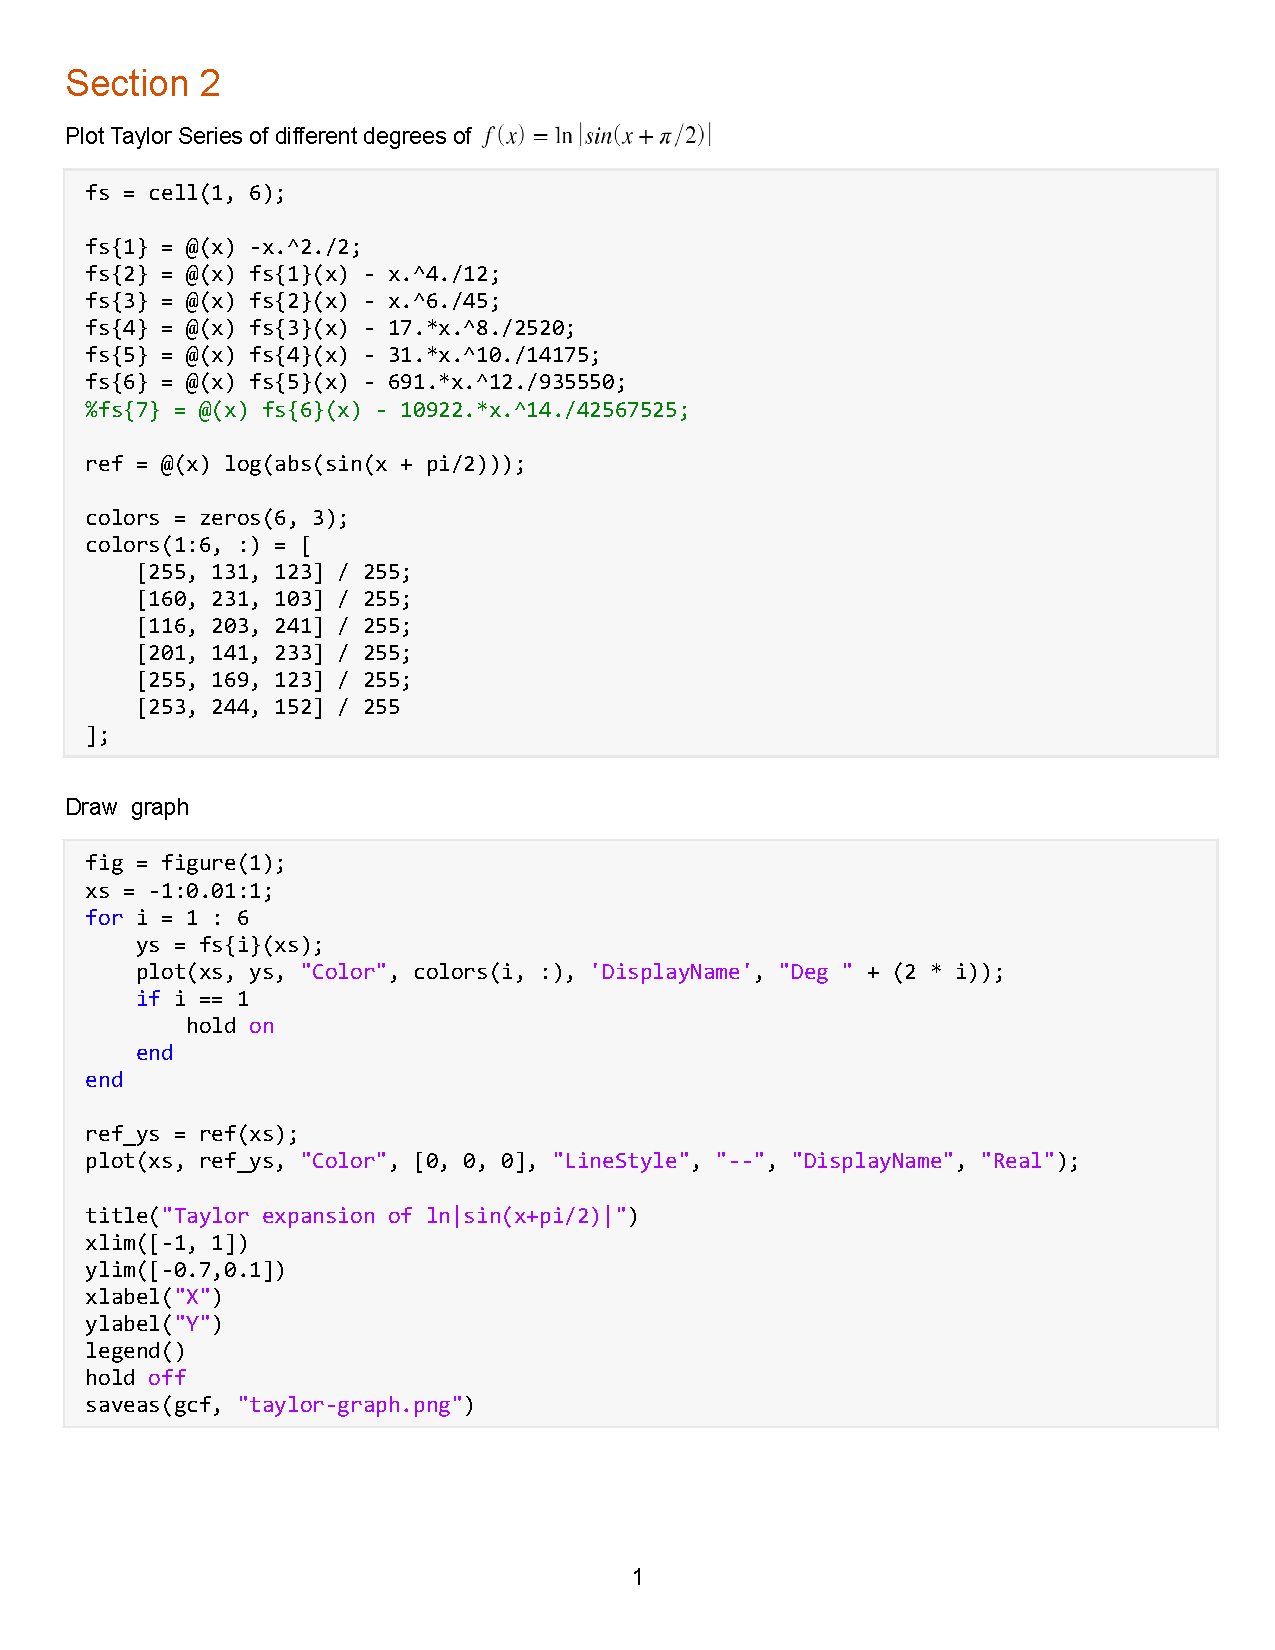
\includepdf[pages=-]{MatlabTaylor.pdf}

\end{document}
